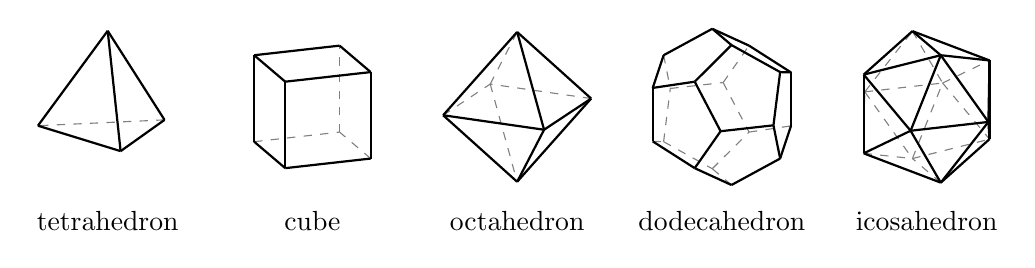
\begin{tikzpicture}[line join=round]
  % tetrahedron
  \draw[dashed, gray] (0.722,-0.165) -- (-0.886,-0.239);
  \draw[thick] (-0.000,0.966) -- (0.164,-0.562);
  \draw[thick] (-0.000,0.966) -- (0.722,-0.165);
  \draw[thick] (-0.000,0.966) -- (-0.886,-0.239);
  \draw[thick] (0.164,-0.562) -- (0.722,-0.165);
  \draw[thick] (0.164,-0.562) -- (-0.886,-0.239);
  \node at (0.00,-1.45) {tetrahedron};
  % cube
  \draw[dashed, gray] (1.860,-0.442) -- (2.945,-0.320);
  \draw[dashed, gray] (3.340,-0.656) -- (2.945,-0.320);
  \draw[dashed, gray] (2.945,-0.320) -- (2.945,0.778);
  \draw[thick] (2.255,-0.778) -- (2.255,0.320);
  \draw[thick] (2.255,-0.778) -- (1.860,-0.442);
  \draw[thick] (2.255,-0.778) -- (3.340,-0.656);
  \draw[thick] (2.255,0.320) -- (1.860,0.656);
  \draw[thick] (2.255,0.320) -- (3.340,0.442);
  \draw[thick] (1.860,-0.442) -- (1.860,0.656);
  \draw[thick] (1.860,0.656) -- (2.945,0.778);
  \draw[thick] (3.340,-0.656) -- (3.340,0.442);
  \draw[thick] (3.340,0.442) -- (2.945,0.778);
  \node at (2.60,-1.45) {cube};
  % octahedron
  \draw[dashed, gray] (6.140,0.106) -- (4.858,0.290);
  \draw[dashed, gray] (4.260,-0.106) -- (4.858,0.290);
  \draw[dashed, gray] (4.858,0.290) -- (5.200,0.951);
  \draw[dashed, gray] (4.858,0.290) -- (5.200,-0.951);
  \draw[thick] (6.140,0.106) -- (5.542,-0.290);
  \draw[thick] (6.140,0.106) -- (5.200,0.951);
  \draw[thick] (6.140,0.106) -- (5.200,-0.951);
  \draw[thick] (4.260,-0.106) -- (5.542,-0.290);
  \draw[thick] (4.260,-0.106) -- (5.200,0.951);
  \draw[thick] (4.260,-0.106) -- (5.200,-0.951);
  \draw[thick] (5.542,-0.290) -- (5.200,0.951);
  \draw[thick] (5.542,-0.290) -- (5.200,-0.951);
  \node at (5.20,-1.45) {octahedron};
  % dodecahedron
  \draw[dashed, gray] (6.922,-0.438) -- (7.060,-0.442);
  \draw[dashed, gray] (7.060,-0.442) -- (7.145,0.234);
  \draw[dashed, gray] (7.060,-0.442) -- (7.678,-0.785);
  \draw[dashed, gray] (7.060,0.656) -- (7.145,0.234);
  \draw[dashed, gray] (7.145,0.234) -- (7.816,0.309);
  \draw[dashed, gray] (7.922,-0.992) -- (7.678,-0.785);
  \draw[dashed, gray] (7.678,-0.785) -- (8.145,-0.320);
  \draw[dashed, gray] (7.816,0.309) -- (8.145,-0.320);
  \draw[dashed, gray] (7.816,0.309) -- (8.145,0.778);
  \draw[dashed, gray] (8.145,-0.320) -- (8.678,-0.241);
  \draw[thick] (6.922,-0.438) -- (6.922,0.241);
  \draw[thick] (6.922,-0.438) -- (7.455,-0.778);
  \draw[thick] (6.922,0.241) -- (7.455,0.320);
  \draw[thick] (6.922,0.241) -- (7.060,0.656);
  \draw[thick] (7.455,-0.778) -- (7.784,-0.309);
  \draw[thick] (7.455,-0.778) -- (7.922,-0.992);
  \draw[thick] (7.455,0.320) -- (7.784,-0.309);
  \draw[thick] (7.455,0.320) -- (7.922,0.785);
  \draw[thick] (7.060,0.656) -- (7.678,0.992);
  \draw[thick] (7.784,-0.309) -- (8.455,-0.234);
  \draw[thick] (7.922,-0.992) -- (8.540,-0.656);
  \draw[thick] (7.922,0.785) -- (7.678,0.992);
  \draw[thick] (7.922,0.785) -- (8.540,0.442);
  \draw[thick] (7.678,0.992) -- (8.145,0.778);
  \draw[thick] (8.455,-0.234) -- (8.540,-0.656);
  \draw[thick] (8.455,-0.234) -- (8.540,0.442);
  \draw[thick] (8.540,-0.656) -- (8.678,-0.241);
  \draw[thick] (8.540,0.442) -- (8.678,0.438);
  \draw[thick] (8.145,0.778) -- (8.678,0.438);
  \draw[thick] (8.678,-0.241) -- (8.678,0.438);
  \node at (7.80,-1.45) {dodecahedron};
  % icosahedron
  \draw[dashed, gray] (9.601,-0.590) -- (9.615,0.191);
  \draw[dashed, gray] (9.601,-0.590) -- (10.220,-0.656);
  \draw[dashed, gray] (9.601,0.410) -- (9.615,0.191);
  \draw[dashed, gray] (9.615,0.191) -- (10.220,-0.656);
  \draw[dashed, gray] (9.615,0.191) -- (10.220,0.962);
  \draw[dashed, gray] (9.615,0.191) -- (10.603,0.303);
  \draw[dashed, gray] (10.580,-0.962) -- (10.220,-0.656);
  \draw[dashed, gray] (10.220,-0.656) -- (10.603,0.303);
  \draw[dashed, gray] (10.220,-0.656) -- (11.199,-0.410);
  \draw[dashed, gray] (10.220,0.962) -- (10.603,0.303);
  \draw[dashed, gray] (10.603,0.303) -- (11.199,-0.410);
  \draw[dashed, gray] (10.603,0.303) -- (11.199,0.590);
  \draw[thick] (9.601,-0.590) -- (9.601,0.410);
  \draw[thick] (9.601,-0.590) -- (10.197,-0.303);
  \draw[thick] (9.601,-0.590) -- (10.580,-0.962);
  \draw[thick] (9.601,0.410) -- (10.197,-0.303);
  \draw[thick] (9.601,0.410) -- (10.580,0.656);
  \draw[thick] (9.601,0.410) -- (10.220,0.962);
  \draw[thick] (10.197,-0.303) -- (10.580,-0.962);
  \draw[thick] (10.197,-0.303) -- (10.580,0.656);
  \draw[thick] (10.197,-0.303) -- (11.185,-0.191);
  \draw[thick] (10.580,-0.962) -- (11.185,-0.191);
  \draw[thick] (10.580,-0.962) -- (11.199,-0.410);
  \draw[thick] (10.580,0.656) -- (10.220,0.962);
  \draw[thick] (10.580,0.656) -- (11.185,-0.191);
  \draw[thick] (10.580,0.656) -- (11.199,0.590);
  \draw[thick] (10.220,0.962) -- (11.199,0.590);
  \draw[thick] (11.185,-0.191) -- (11.199,-0.410);
  \draw[thick] (11.185,-0.191) -- (11.199,0.590);
  \draw[thick] (11.199,-0.410) -- (11.199,0.590);
  \node at (10.40,-1.45) {icosahedron};
\end{tikzpicture}
